
\begin{figure}[H]
    \centering
    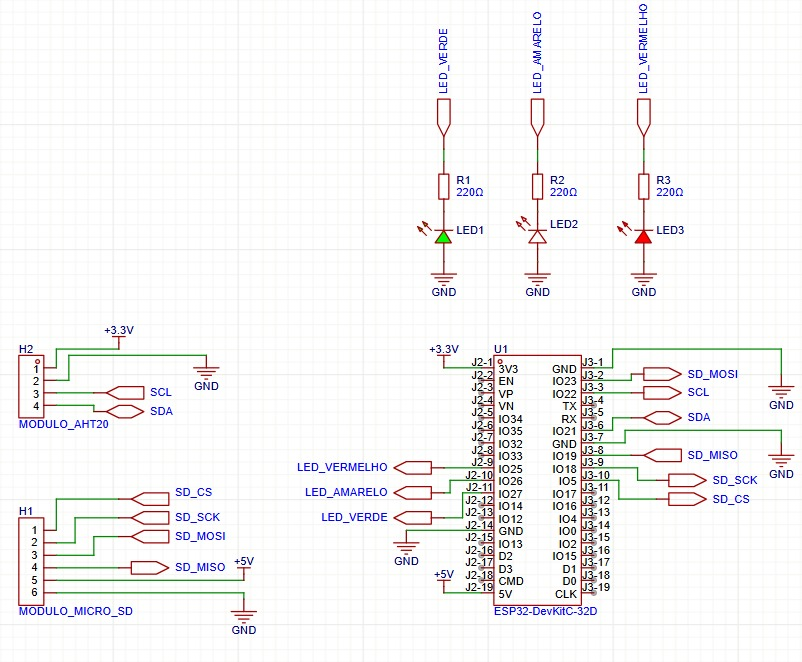
\includegraphics[width=1.0\textwidth]{img_arquivo/Esquematico.png} 
    \caption{Esquemático de Hardware}
    \label{fig:modelagem_de_circuitos}
\end{figure}

O diagrama elétrico detalha as conexões físicas entre o microcontrolador ESP32 e os periféricos do sistema. Nele, destaca-se a integração do sensor AHT20 via barramento I2C e a interface do módulo microSD via protocolo SPI. Além disso, o esquema apresenta o circuito de sinalização visual, composto por três LEDs (Verde, Amarelo e Vermelho) equipados com resistores de 220 $\Omega$ para garantir a proteção das portas lógicas do chip